% !TeX spellcheck = en_US

% TeX'ing this file requires that you have all prerequisites
% for REVTeX 4.1 installed
%
% See the REVTeX 4 README file
% It also requires running BibTeX. The commands are as follows:
%
%  1)  latex templateForReport.tex
%  2)  bibtex templateForReport
%  3)  latex templateForReport.tex
%  4)  latex templateForReport.tex
%
\documentclass[%
reprint,
%superscriptaddress,
%groupedaddress,
%unsortedaddress,
%runinaddress,
%frontmatterverbose,
%preprint,
%showpacs,preprintnumbers,
%nofootinbib,
%nobibnotes,
%bibnotes,
amsmath,amssymb,
aps,
pra,
%prb,
%rmp,
%prstab,
%prstper,
floatfix,
]{revtex4-2}

%\usepackage{fontspec}
%\usepackage{unicode-math}
\usepackage[english]{babel}

%\usepackage{polyglossia}

\usepackage{graphicx}% Include figure files
\usepackage{subcaption}% For subfigures
\usepackage{dcolumn}% Align table columns on decimal point
\usepackage{booktabs}% for nicer tables
\usepackage[separate-uncertainty]{siunitx}[=v2]
\usepackage{enumitem}% for letters in enumerations
\usepackage{csquotes}


\usepackage{tikz}% For nice drawings
\usepackage{pgf}% data visualization
\usetikzlibrary{angles,quotes,calc,intersections,through,backgrounds, babel, positioning}

\usepackage{hologo}% for the TeX logo
\usepackage{natbib}

\usepackage{amsmath}
\usepackage{amsfonts}
\usepackage{physics}% easys power notation and add more functions
\usepackage[utf8]{inputenc}

\usepackage{mathtools}

\usepackage{hyperref}% add hypertext capabilities
%\usepackage{pgfcache}
%\setpgfpreamble{\usepackage[separate-uncertainty]{siunitx}}

\usepackage{defs}

%\DeclareSIUnit \div {div}
%\setdefaultlanguage{german}
\sisetup{locale = DE}
\setlist{itemsep=3pt,parsep=0pt}

\begin{document}
	\title{Notes for \enquote{GRAVITATION} - MTW}
	
	\author{Nico Dichter}
	\email{nicodichter@nocoffeetech.de}
	
	\affiliation{Friedrich-Wilhelm-Universität Bonn}
	
	% It is always \today, today, but any date may be explicitly specified
	\date{\today}
	
	\begin{abstract}
		abc
	\end{abstract}
	
	\maketitle
	
	%\thesection{Introduction}\label{sec:introduction}
	
	
	\section{Geometrodynamics in Brief}\label{sec:chapter1}


\subsection{The parable of the apple}\label{susec:1_1}
Space tells matter how to move and matter tells space how to curve.

\subsection{Spacetime with and without coordinates}\label{susec:1_2}
\subsubsection{\hint for possible different characterization \page{6}}

\enquote{But with all the daring in the world, how is one to drive a nail into spacetime to mark a point? Happily, nature provides its own way to localize a point in spacetime, as Einstein was the first to emphasize. Characterize the point by what happens there!}

\subsubsection{\hint from idealized limit \page{10}}

\enquote{A more detailed diagram would show a maze of world line and of light rays and the intersections between them. From such a picture, one can in imagination step to the \emph{idealized} limit: an infinitely dense collection of light rays and of world lines of infinitesimal test particles.}

\subsubsection{\hint of breakdown of manifold description \page{12}}
\enquote{Not so quantum general relativity or \enquote{quantum geometrodynamics}. It predicts violent fluctuations in the geometry at distances on the order of the Planck length,\dots As nearly as one can estimate these fluctuations give space at small distances a \enquote{multiply connected} or \enquote{foam-like} character.}

\subsection{Weightlessness}\label{susec:1_3}
\subsubsection{\cbox{1.2} \page{16}}
\paragraph{Lorand von Eötvös \page{16}}
\begin{figure}[htb]
	\centering
	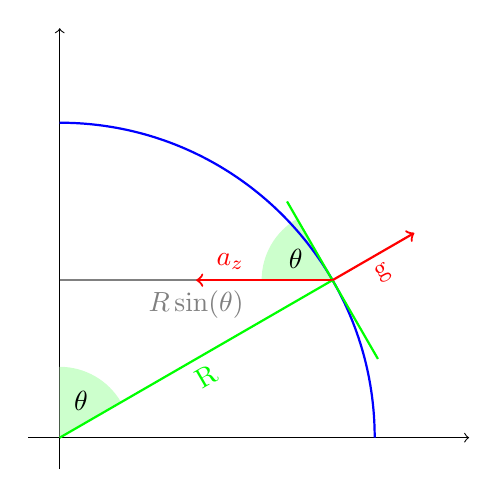
\begin{tikzpicture}
		\def\r{4} % radius
		\def\ang1{30}
		\def\q{{\r/cos(\ang1)}}
		\def\t{{\r*sin(\ang1)}}
		\def\zt{0.5}
		\coordinate (A) at (\ang1:1cm);
		\coordinate (C) at (0,1);
		\coordinate (B) at (0,0);
		
		\draw[->] (0,-0.1*\r) -- (0,1.3*\r);
		\draw[->] (-0.1*\r,0) -- (1.3*\r,0);
		
		\draw pic [fill=green!20, angle radius=9mm,
		"$\theta$"] {angle = A--B--C};
		
		\coordinate (O) at (0,0); % circle center O	
		\coordinate (Q) at (\q,0); % external point Q
		\coordinate (P) at (\ang1:\r); % point of tangency, P
		\coordinate (R) at (0,\t); % y intercept of P
		\coordinate (T) at ($(Q)!1.3!(P)$); % y intercept of P
		
		\draw pic [fill=green!20, angle radius=9mm,
		"$\theta$"] {angle = T--P--R};
		
		\draw [blue,thick](\r,0mm) arc [start angle=0, end angle=90, radius=\r];
		\draw[green,thick] ($(Q)!0.5!(P)$) -- ($(Q)!1.5!(P)$);
		\draw[green,thick] (O) --node[midway,sloped,below] {R} (P);
		\draw[gray,thick] (R) --node[midway,sloped,below] {$R\sin(\theta)$} (P);
		\draw[->, red, thick] (P) -- node[midway,sloped,below] {g}($(P)!-0.3!(O)$);
		\draw[->, red, thick] (P) -- node[near end,sloped,above] {$a_z$}($(P)!\zt!(R)$);
		
		%\fill[red] (O) circle(0.05) node[below right] {O};
		%\fill[red] (Q) circle(0.05) node[below left] {Q};
		%\fill[red] (P) circle(0.05) node[above,right=0.2cm] {P};
		%\fill[red] (R) circle(0.05) node[above] {R};
	\end{tikzpicture}
	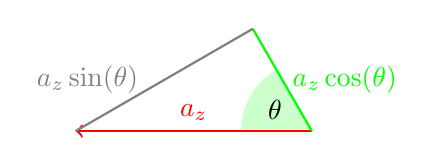
\begin{tikzpicture}[rotate=90]
		
		\def\r{3} % radius
		\def\ang1{30}
		
		\coordinate (O) at (0,0); 
		\coordinate (P) at (0,\r);
		\coordinate (Q) at (\ang1:{\r*sin(\ang1)});
		
		\draw pic [fill=green!20, angle radius=9mm,
		"$\theta$"] {angle = Q--O--P};
		
		\draw[->, red, thick] (O) -- node[midway,above] {$a_z$}(P);
		\draw[green,thick] (O) --node[midway,above,right] {$a_z\cos(\theta)$} (Q);
		\draw[gray,thick] (P) --node[midway,above, left=0.2] {$a_z\sin(\theta)$} (Q);
	\end{tikzpicture}
	\caption{Forces mentioned in \cbox{1.2},  \emph{Lorand von Eötvös}, where $R$ is the radius of the earth and $\theta$ is the angle measured from the north pole}
	\label{fig:1_3_1}
\end{figure}

The forces mentioned are shown in \reffig{1_3_1}, from which we directly observe that the centripetal acceleration is in total
\[a_z=\omega^2 R \sin(\theta),\]
which is \emph{independent} of $g$ in this way of viewing forces ($\omega$ is the rotation speed of the earth).
From this we get the northward directed part of $a_z$  to be 

\[a_z \cos(\theta)=\omega^2 R \sin(\theta)\cos(\theta).\]

\paragraph{Beall \page{17}}
We know the highest observed energies of the myon to be \[E_\mu = \SI{1e13}{\electronvolt}.\]
While the upper threshold is mentioned to be \[E_{\text{thresh}}=\num{1e3} m c^2\].
If now the myon were to be \enquote{too light} we would have \[E_\mu>E_{\text{thresh}}.\]

On the other hand we know the highest observed energies of photons to be \[E_\gamma=\SI{1e13}{\electronvolt}.\]
The transferred energy (to a photon) mentioned results in \[E_\gamma\geq 2 m c^2.\] These two observations combined put an upper limit (Not \enquote{too heavy}) on $m$.

\subsubsection{\enquote{This assumption of exact physical equivalence makes it impossible for us to speak of the absolute acceleration of the system of reference, \dots} \page{17}}
This because any part of the acceleration could be due to a gravitational field.


\subsection{Local Lorentz Geometry, with and without Coordinates}\label{susec:1_4}
\subsubsection{\hint: What about breakdown at small scales? \page{21}}
\enquote{The geometry of spacetime is locally Lorentzian everywhere.}

\subsection{Time}\label{susec:1_5}
Time is defined so that motion looks simple.

\subsection{Curvature}\label{susec:1_6}
\subsubsection{\cbox{1.6} \page{32}}
\paragraph{Figure C \page{33}}
The formula \[r=\dfrac{d^2}{8 a},\]
where $r$ is the radius of curvature, $d$ is the \enquote{direct} distance between start and end point 
and $a$ is the raise of the track of e.g. the ball, can be derived as follows:

Denote by $\alpha$ the angle inscribed by the shown cone under consideration, then
\begin{equation} 
	\sin(\alpha)=\dfrac{d}{r} \label{eq:1_6_1}
\end{equation}
 Further denote by $x$ the distance between the center of curvature and the intersection point of the radial line at $\alpha/2$ with the \enquote{direct} line of connection between start and end point. Or in formulas \[x=r-a.\]
 Then we know
 \begin{align*} 
 	\cos(\dfrac{\alpha}{2})&=\dfrac{x}{r}\\
	\Rightarrow a&=r-x\\
	&=r\left(1-\cos(\dfrac{\alpha}{2})\right)\\
	&\overset{\crefeq{1_6_1}}{\approx}r\left(1-\sqrt{1-\left(\dfrac{d}{2r}\right)^2}\right)\\
	&\approx r\left(1-\left(1-\dfrac{d^2}{8r^2}\right)\right)\\
	&=\dfrac{d^2}{8r}\\
	\Rightarrow r &=\dfrac{d^2}{8a}
 \end{align*}

\subsubsection{\eq{1.13} \page{37}}
The summation only happens over the spatial components i.e. $j$ because we are here considering $v\ll c$, such that the separation in the time coordinate is negligible.


\subsection{Effect of Matter on Geometry}\label{susec:1_7}
\subsubsection{\cbox{1.9} \page{38}}
\paragraph{Galileo Galilei (1638)}
What is meant here is uniform acceleration leading to
\[s=\dfrac{1}{2}a t^2 \Rightarrow s \propto t^2.\]

\subsubsection{\hint: GR only being valid for larger (average) scales? \page{42}}
\enquote{the field equation shows how the stress-energy of matter generates an \emph{average} curvature in its neighborhood.}

\subsubsection{\exercise{1.1} \page{44}}
By unrolling the cylinder it is obvious that geodesics, which are parallel at one point, are parallel at any other point, i.e. they suffer no geodesic deviation:
\begin{align*} 
	\derivative{^2\xi}{s^2}&=0\overset{\eq{1.6}}{=}-R\xi\\
	\Rightarrow R&=0
\end{align*}
Given the formula \[R=\dfrac{1}{\varrho_1\varrho_2},\]
where $\varrho_i$ are the principal radii of curvature at the point in question.
We then get for a cylinder \[\varrho_1=\infty\qquad\varrho_2=r \quad\Rightarrow R=0,\]
where $r$ is the radius of the cylinder in the 3-dimensional euclidean embedding space.
\subsubsection{\exercise{1.2} \page{44}}
Using \eq{1.14} the values in question can be calculated.

\subsubsection{\exercise{1.3} \page{44}}
First fix some notation:
\begin{align*} 
	M&=\text{Mass of satellite}\\
	\omega&=\text{Angular frequency of satellite}\\
	r&=\text{Radius of orbit of satellite}\\
	m&=\text{Mass of central object}\\
	\varrho_{\text{Kepler}}&=\dfrac{m}{\frac{4\pi}{3}r^3}=\text{Kepler density}
\end{align*}
By setting the centripetal acceleration of the satellite equal to the gravitational acceleration (in Newtonian mechanics), we get:
\begin{align*} 
	M\omega^2 r&= G\dfrac{m M}{r^2}\\
	\Rightarrow \omega^2&=G\dfrac{m}{r^3}=\dfrac{4\pi G}{3}\varrho_{\text{Kepler}}
\end{align*}


	\section{Foundations of Special Relativity}\label{sec:chapter2}

\subsection{Quantum Mechanics}\label{susec:2_1}

\subsection{Symmetries}\label{susec:2_2}
\subsubsection{\enquote{For this to be unitary and linear, $t$ must be Hermitian and linear} \page{51}}\label{sususec:2_2_p51_1}
Linearity is trivial and hermiticity follow from the following observation:
\begin{align*} 
	\innerproduct{U\Psi}{U\Phi}=&\innerproduct{(1+i\varepsilon t) \Psi}{(1+i\varepsilon t) \Phi}\\
	=&\innerproduct{\Psi}{\Phi}+\varepsilon i\left(\innerproduct{\Psi}{t \Phi}-\innerproduct{t\Psi}{ \Phi}\right)+\order{\varepsilon^2}\\
	\overset{\eq{2.2.2}}{\Leftrightarrow}&\innerproduct{\Psi}{t \Phi}=\innerproduct{t\Psi}{\Phi}\\
	\overset{\eq{2.1.5}}{\Leftrightarrow}&t^\dagger=t
\end{align*}

\subsubsection{\eq{2.2.19} \page{54}}
$f^a_{bc}$ and $f^a$ have to be real as $\theta^a$ are real.


	\section{Scattering Theory}\label{sec:chapter3}

\subsection{"In" and "Out" States}\label{susec:3_1}
	%\cleardoublepage
	%\newpage
	%\input{4-daten.tex}
	
	\begin{acknowledgments}
		Typesetting done with \emph{REV\TeX\ 4.2}.
	\end{acknowledgments}
	
	
	%\newpage
	
	%\listoffigures
	%\listoftables
	
	% Add the bibliography file
	\bibliography{bibliography}
	%\clearpage
	
	%\appendix
	
	%\input{7-anhang.tex}
\end{document}